%%%%%%%%%%%%%%%%%%%%%%%%%%%%%%%%%%%%%%%%%%%%%%%%%%%
%% P3: Phenomenology of Particle Physics                         
%%
%% Author:  André Rubbia                   		 
%%
%% Figure 11.20 Kinetic-energy distribution of the recoil electron in Compton scattering for several incident photon energies.
%%
%% This work is licensed under the Creative Commons Attribution 4.0 International License. 
%% To view a copy of this license, visit http://creativecommons.org/licenses/by/4.0/ or 
%% send a letter to Creative Commons, PO Box 1866, Mountain View, CA 94042, USA.
%%
%%%%%%%%%%%%%%%%%%%%%%%%%%%%%%%%%%%%%%%%%%%%%%%%%%%

\documentclass[a4paper,10pt]{article}

\usepackage[T1]{fontenc}
\usepackage[utf8]{inputenc}
\usepackage{lmodern}
\usepackage[labelfont=bf]{caption}
\usepackage{upgreek}

\usepackage{tikz}
\usepackage{pgfplots}
\pgfplotsset{compat=1.17}
\usepgfplotslibrary{ternary}
\usepgfplotslibrary{fillbetween}
\usepgfplotslibrary{external}

\usepackage{braket}

\def\d{\mathrm{d}}

\begin{document}

%%%%%%%%%%%%%%%%% FIGURE %%%%%%%%%%%%%%%%%%%%%%%%%%%%%%%%%%
\begin{figure}[htb]
\begin{center}
\pgfplotsset{every axis/.append
    style={
    line width=1pt,
    tick style={line width=0.8pt}}}
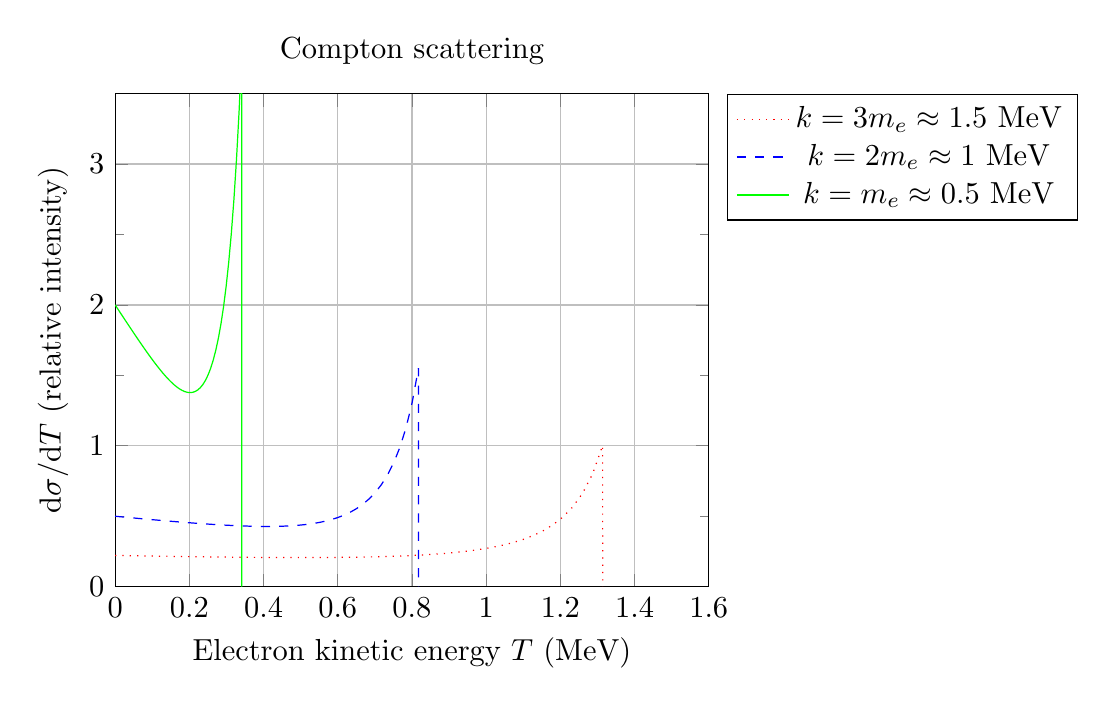
\begin{tikzpicture}[scale=1.1]
    \begin{axis}[
        title=Compton scattering,
        xlabel={Electron kinetic energy $T$ (MeV)},
        ylabel={$\d \sigma/\d T$ (relative intensity)},
        xmin=0, xmax=1.6,
        ymin = 0, ymax=3.5,
        minor y tick num=1,
        grid = major,
        legend entries={
        $k=3m_e\approx 1.5$~MeV,
        $k=2m_e\approx 1$~MeV,
        $k=m_e\approx 0.5$~MeV,
        },
                legend style={legend pos = outer north east}
    ]
        \addplot [red,samples=50,domain=0:1.314, dotted]
        {(2+(x/1.5)^2/((3^2)*(1-(x/1.5))^2)+(x/1.5)*((x/1.5)-2/3)/(1-(x/1.5)))/(3^2)} -- (1.314,0);
        \addplot [blue,samples=50,domain=0:0.8176, dashed]
        {(2+x^2/((2^2)*(1-x)^2)+x*(x-2/2)/(1-x))/(2^2)} -- (0.8176,0);
        \addplot [green,samples=50,domain=0:0.341]
        {(2+(x/0.5)^2/((1^2)*(1-x/0.5)^2)+(x/0.5)*((x/0.5)-2/1)/(1-(x/0.5)))/(1^2)} -- (0.341,0);
   \end{axis}
\end{tikzpicture}%
\caption{Kinetic-energy distribution of the recoil electron in Compton scattering for
several incident photon energies.}
\end{center}
\end{figure}
%%%%%%%%%%%%%%%%% END FIGURE %%%%%%%%%%%%%%%%%%%%%%%%%%%%%%
%

\end{document}
